\begin{figure}[t]
\centering
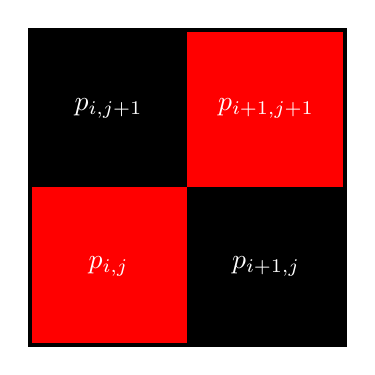
\begin{tikzpicture}[scale=1]
\draw[ultra thick, fill=red] (0,0) rectangle (4,-4);
    \foreach \row in {0,1} {
        \foreach \column in {0} {
    \fill ({4*\column + mod(\row,2)*2}, -\row*2) rectangle +(2,-2);
        }
    }
% \matrix (m) at (0,0) [matrix of nodes,nodes={},
%   anchor=north west,column sep={2cm,between origins},
%   row sep={2cm,between origins}] {
%  {\color{white}{$p_{i,j+1}$}} & {$p_{i+1,j+1}$} \\
%  {$p_{i,j}$} & {\color{white}{$p_{i+1,j}$}} \\
% };
\node at (1,-1) {\color{white}{$\bm{p_{i,j+1}}$}};
\node at (1,-3) {\color{white}{$\bm{p_{i,j}}$}};
\node at (3,-1) {\color{white}{$\bm{p_{i+1,j+1}}$}};
\node at (3,-3) {\color{white}{$\bm{p_{i+1,j}}$}};

% \matrix[matrix of nodes,nodes={draw}]{A & B & C & D & E\\f & G & H & I & J};
\end{tikzpicture}
    \caption{Example checkerboard pattern used for red/black splitting}
    \label{fig:redblack_checkerboard}
\end{figure}